% \setcounter{figure}{0}
% \setcounter{listing}{0}

\pagenumbering{arabic}
\renewcommand*{\thepage}{B-\arabic{page}}



\chapter{Description of Digital Submission}
\label{cha:Description of Digital Submission}
\label{chapter:digital-medium}

\textbf{Thesis Evidence Number:} \\ \myEvidenceNumber

The content of the electronic medium (data and models), which exceeds \texttt{1GB} is submitted to the thesis supervisor ... %(doc. Ing. Giang Nguyen Thu, PhD.).

\textbf{Name of the submitted archive:}\\ \texttt{BP\_MenoPriezvisko.zip}

The digital part included in the thesis contains the following files:
\begin{itemize}
    \item Ubuntu OS: run in command line \texttt{\$ tree} to get a directory structure as below.
    \item Inspiration from \textit{https://github.com/FIIT-ISA/cookiecutter-data-science}
\end{itemize}


\begin{verbatim}
    ROOT // Root directory.
    │
    ├── flatbuffers // This flatbuffers director
    └── scheme
\end{verbatim}

\begin{figure}[H]
    \begin{centering}
    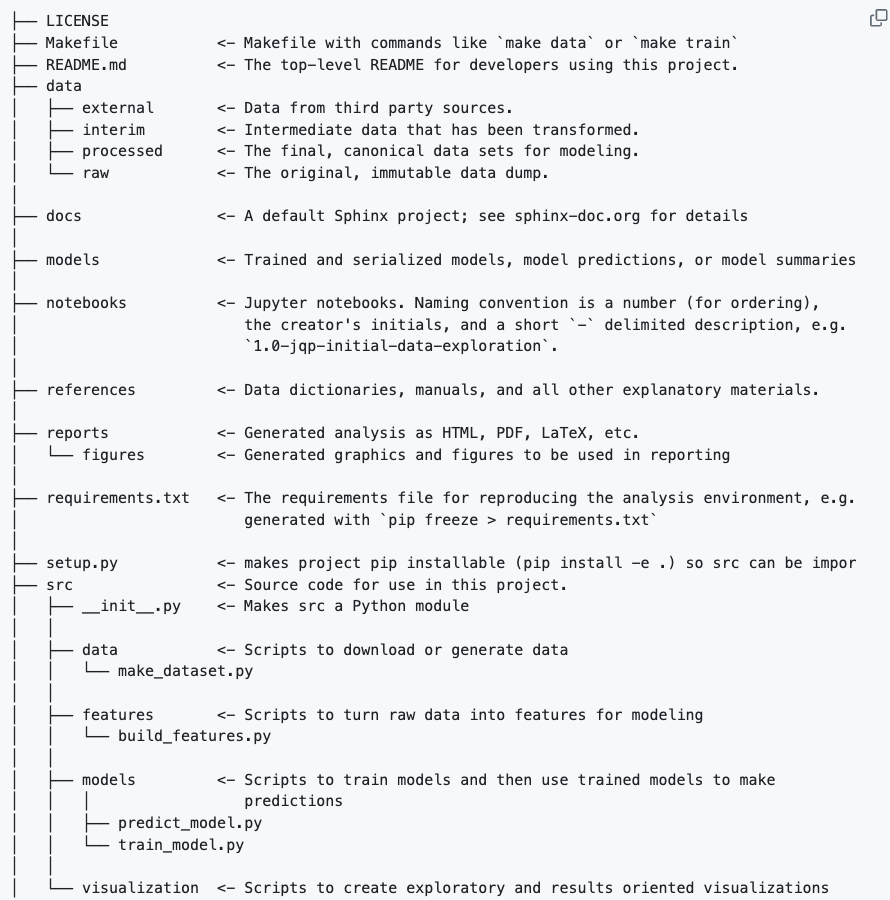
\includegraphics[width=\textwidth]{appendices/zip-file-structure.png}
    \par\end{centering}
\caption{The structure of the ZIP file \label{fig:zip-file-structure}}
\end{figure}



\chapter{Technical Documentation}
\label{chapter:Technical-Documentation}

\section{Setup}
\label{sec:appendix-setup}

hardware: examples are in Table~\ref{table:experiments_environment} \\
software: libraries, versioning, \\
virtual environments, ... \\
datasets, \\
NDA, ...\\
others ...


\begin{table}[h!]
    \centering
    \footnotesize
    \begin{tabular}{lccccc}
    \toprule
Machine & Remote    & Google Colab  & Kaggle    & FIIT Cloud    & Local    \\ 
    \midrule
Python      & 3.9.19        & 3.10.12        & - & -    & 3.10.12        \\
PyTorch     & -             & -              & - & -    & -              \\
TensorFlow  & 2.10          & 2.15           & - & -    & 2.14           \\
GPU (NVIDIA) & RTX xx & Tesla T4 15 GB & Tesla P100 16GB & - & -      \\
CUDA        & 12.2          & 12.2           & - & -    & -              \\
cuDNN       & 8.1.0         & N/A            & - & -    & -              \\
CUDA Toolkit & 11.2.2       & N/A            & - & -    & -              \\ 
RAM    & 32/64 GB        & 51 GB & 30 GB     & 32 GB    & 16 GB         \\
CPU  & 8x cores Intel i7   & -  & Xeon 4x cores & 4x cores & -              \\
Storage    & SSD  & Google Driver  & 73 GB & 128 GB & HDD            \\
    \bottomrule
    \end{tabular}
    \caption{Hardware, software and versioning used for realization}
    \label{table:experiments_environment}
\end{table}

IDC Lab (Intelligent Data Computing), IDSA~\footnote{Intelligent Data and Systems with Applications (IDSA) research group~\url{https://idsa.fiit.stuba.sk/} } at FIIT STU in Bratislava.



\section{Installation Manual}
\label{sec:Installation-Manual}

Example:
\begin{enumerate}
    \item Clone the project from the Git repository (URL) OR unzip the ZIP file ...
    \item Run \emph{pip install -r requirements.txt} in the root folder of the project
    \item Run \emph{python -m spacy download en} to have the data corpus ...
\end{enumerate}



\section{User's Manual}
\label{sec:User-Manual}

Example:
\begin{enumerate}
    \item The program is launched via the main Python file \emph{main.py} using the command \emph{python main.py}. 
    
    \item After starting the program, a graphical user interface is displayed, where summarization for a single input file can be initiated directly from the main screen.

    \item The buttons at the top of the screen allow navigation between the program’s functionalities, such as multi-file summarization or article viewing. On these screens, the \emph{Back to main menu} button can be used to return to the main screen.
\end{enumerate}


Screenshot(s) of the user graphical interface (GUI) as an image (Figure)

Another variant for a work without GUI:\\
The main objective of this work is to ... 
Several case studies were presented that examine the capabilities of ... to show the feasibility and achievability of ... 
Users in our work are considered to work directly with the code as described in Section~\ref{sec:Installation-Manual}.



\section{Developer Manual}
\label{sec:Developer-Manual}

if needed then add this Section